\documentclass[12pt, a4paper]{article}

\usepackage[utf8]{inputenc}
\usepackage[T1]{fontenc}
\usepackage[english]{babel}
\usepackage{lmodern}
\usepackage[a4paper, margin=1in]{geometry}
\usepackage{microtype}
\linespread{1.2}
\usepackage{titling}
\usepackage[colorlinks=true,linkcolor=blue,citecolor=blue,urlcolor=blue]{hyperref}
\usepackage{amsmath, amssymb}
\usepackage{graphicx}
\usepackage{caption}
\usepackage{subcaption}
\usepackage{listings}
\usepackage{xcolor}
\usepackage{enumitem} 

\definecolor{codegray}{rgb}{0.4,0.4,0.4}
\definecolor{codegreen}{rgb}{0,0.5,0}
\definecolor{codeblue}{rgb}{0,0,0.7}

\lstdefinestyle{mystyle}{
  basicstyle=\ttfamily\small,
  commentstyle=\color{codegreen},
  keywordstyle=\color{codeblue}\bfseries,
  stringstyle=\color{codegray},
  numberstyle=\tiny\color{gray},
  numbers=left,
  stepnumber=1,
  breaklines=true,
  frame=single,
  backgroundcolor=\color{gray!10}
  rulecolor=\color{gray!50} 
}
\lstset{style=mystyle}


\pretitle{\begin{center}\LARGE\bfseries}
\posttitle{\end{center}\vskip 0.5em}

\title{CS1301x Revision Note\\
\Large Computing in Python IV:\\
\large Objects \& Algorithms\\
\normalsize (unoffical personal note)}

\date{\today}
\author{kayikc @}
\begin{document}
\maketitle
\tableofcontents
\pagebreak
\section{Algorithms}

Computers excel at quickly performing complex math.  Machine learning, for instance, combines statistics with powerful hardware to handle massive calculations.  This exemplifies the "algorithmic" side of computer science.  An algorithm is simply a defined series of steps transforming input into output.

\textbf{Examples in Daily Life:}
\begin{itemize}
    \item Data compression
    \item Random number generation
    \item Search algorithms
\end{itemize}



\section{Complexity and Big O Notation}

The power of automated algorithms lies in chaining steps to solve otherwise impractical problems.  Let's consider searching names in a school roster:

\begin{itemize}
    \item \textbf{Sorted:} Finding "David Joyner" takes fewer than 10 checks using binary search.
    \item \textbf{Unsorted:}  Might require up to 500 checks, one by one.
\end{itemize}

Finding duplicates is even trickier:

\begin{itemize}
    \item \textbf{Sorted:}  Around 500 checks (comparing neighbors).
    \item \textbf{Unsorted:}  Could take 125,000 checks (every name against all others).
\end{itemize}

Inefficient algorithms become dramatically slower as data grows. Doubling the students quadruples the work!

Big O notation ($O(\cdot)$) measures how an algorithm's workload increases with data size ($n$).  It focuses on the dominant growth factor, ignoring smaller details like constant multipliers.  For instance, $n^2/2$ simplifies to $O(n^2)$. We care about the scaling trend, not minor optimizations.

\textbf{Common Complexities (from fastest to slowest):}
\begin{itemize}[noitemsep] % Reduce space between items
    \item $O(1)$ (Constant):  Same time, regardless of data size (e.g., checking the first list item).
    \item $O(\log n)$ (Logarithmic): Gets relatively faster with larger input (e.g., binary search in a sorted list).
    \item $O(n)$ (Linear): Time grows directly with input (e.g., checking each item once).
    \item $O(n^2)$ (Quadratic): Time grows with the square of the input (e.g., duplicate checks in an unsorted list).
    \item $O(2^n)$ (Exponential): Time doubles with each additional input (e.g., password brute-forcing).
\end{itemize}

Lower complexity means a faster algorithm, especially for large datasets.

\section{Recursion}
The way I think about Recursion:
\begin{enumerate}
    \item Find the base case (simplest form): Identify the smallest, simplest input(s) for which you can directly compute the answer without recursion.
    \item Find the general equation (recursive step): Determine how to express the solution for larger inputs in terms of the solution(s) for smaller, self-similar subproblems.
\end{enumerate}

\subsection{Example: Finding a Route}

Imagine a function \texttt{find\_route(start, end)} that finds a path from a starting point to an end point. Recursively, this might be represented as follows:

\begin{lstlisting}[language=Python, caption={Conceptual Example: Recursive Route Finding}, numbers=none]
find_route(front_door, office_door)

# Breaks down into:
find_route(front_door, stairwell_entrance)
find_route(stairwell_entrance, stairwell_exit)
find_route(stairwell_exit, office_door)

# ...and further:  % Improved comment style
find_route(stairwell_exit, hallway)
find_route(hallway, office_door) 
\end{lstlisting}

The function calls itself with progressively simpler subproblems, eventually reaching a base case (e.g., the start and end points are the same location), where a direct route exists.

\subsection{Simple Example: Factorial}

The factorial of a number $n$ (written $n!$) is the product of all positive integers up to $n$:  $n! = n \times (n-1) \times \cdots \times 1$.  The recursive definition is $n! = n \times (n-1)!$ with a base case of $1! = 1$.

\lstinputlisting[language=Python, caption=Recursive Factorial, firstline=1, lastline=5]{factorial_recursion.py} 


\subsection{Intermediate Example: Fibonacci Series}

The Fibonacci sequence starts with 1, 1 and continues with each number being the sum of the previous two: 1, 1, 2, 3, 5, 8, and so on.  Recursively:

\begin{itemize}
    \item \textbf{Function} \texttt{fibonacci(n)}:
    \item \textbf{If} \(n > 2\): \textbf{return} \texttt{fibonacci(n-1) + fibonacci(n-2)}
    \item \textbf{If} \(n \le 2\): \textbf{return} 1 
\end{itemize}

This simple recursive implementation is inefficient as it recalculates values multiple times (e.g., `fibonacci(4)` calculates `fibonacci(3)` twice). A more efficient approach uses memoization (storing calculated values in a dictionary) to avoid redundant calculations.

\subsection{Advanced Example: Directory Exploration}

Listing all files in nested directories can be done recursively:

\begin{itemize}
    \item \textbf{Function} \texttt{listFiles(directory)}:
    \item List each file in \texttt{directory}.
    \item For each subfolder in \texttt{directory}, call \texttt{listFiles(subfolder)}.
\end{itemize}

This mimics exploring a building: list items in the current room, then open each door and repeat for the new rooms.


\textit{Head vs. Tail Recursion:} Head recursion processes the current level before going deeper (root $\to$ subfolder $\to$ deeper subfolder). Tail recursion processes the deepest levels first, then the current level (deepest $\to$ subfolder $\to$ root).


\section{Sorting Algorithms}

Sorting algorithms arrange items in a list into a specific order, such as ascending order.  They take an unsorted list as input and produce a sorted version as output. These algorithms can sort various data types (numbers, strings, etc.) as long as there's a way to compare elements. Many sorting algorithms exist, each with varying efficiency. We'll use a 10-number list as a running example, prioritizing ease of implementation over computational complexity.

\begin{figure}[h]
    \centering
    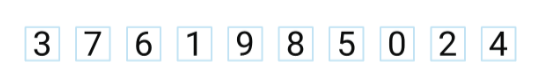
\includegraphics[width=\textwidth]{images/10-number_list.png}
    \caption{The list of 10 unsorted numbers}
    \label{fig:bubble_sort}
\end{figure}

\subsection{Bubble Sort}
`'
\begin{figure}[h]
    \centering
    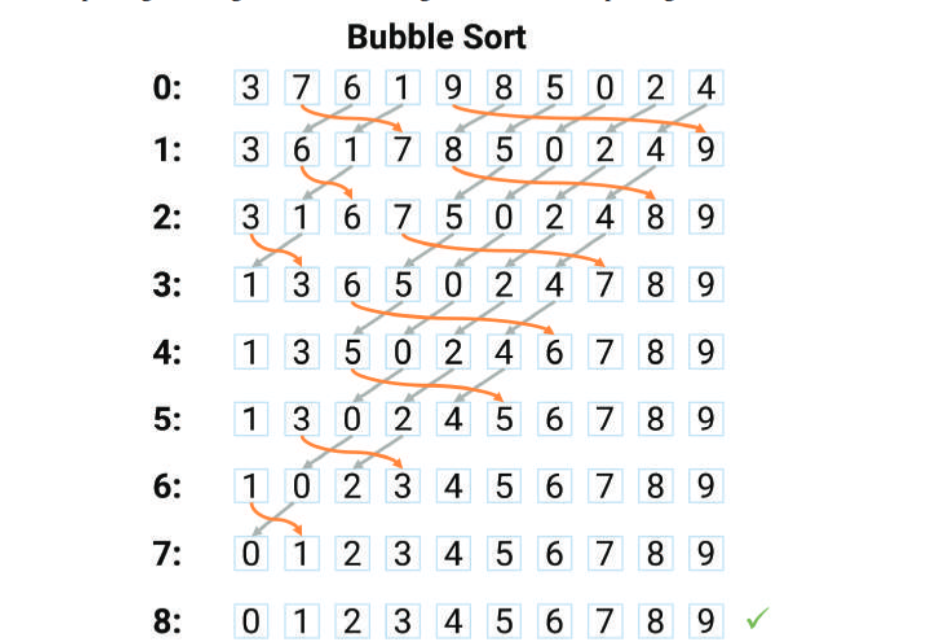
\includegraphics[width=\textwidth]{images/bubble_sort_example.png}
    \caption{Example of Bubble Sort. Orange arrows indicate comparisons and swaps.}
    \label{fig:bubble_sort}
\end{figure}

Bubble sort is a straightforward yet inefficient algorithm. It repeatedly compares adjacent pairs of numbers, swapping them if they're in the wrong order. This process continues until a pass through the list requires no swaps, indicating the list is sorted.

Let's walk through the example in Figure~\ref{fig:bubble_sort}.  The initial list is 3 7 6 1 9 8 5 0 2 4.

\begin{enumerate}
    \item \textbf{Pass 1:}  The algorithm compares 3 and 7 (no swap needed), then 7 and 6 (swap!), 6 and 1 (swap!), 1 and 9 (no swap), and so on.  The largest number, 9, "bubbles" to the end.
    \item \textbf{Pass 2:}  The process repeats.  The second largest number, 8, moves closer to its final position.
    \item \textbf{Subsequent Passes:} This continues.  Each pass places the next largest unsorted number in its correct position.  Notice how smaller numbers gradually "float" towards the beginning (e.g., 0 moves one step forward with each pass).
\end{enumerate}


The orange arrows in Figure~\ref{fig:bubble_sort} show the comparisons and swaps. The algorithm continues until a pass requires no swaps (the last two rows are identical, showing the sorted list).

\textbf{Efficiency:}  Bubble sort has a time complexity of $O(n^2)$.  This means it can be very slow for large lists. In the worst-case scenario (a reverse-sorted list), it performs roughly $n^2$ comparisons.



\subsection{Other Sorting Algorithms (Overview)}

To do


\section{Search Algorithms}

To do

\subsection{Linear Search}

To do

\subsection{Binary Search}

To do


\subsection{Linear vs. Merge Sort + Binary Search}

To do


\end{document}